\documentclass[aspectratio=169]{beamer}
\usetheme{Madrid}
\usecolortheme{default}

% Packages
\usepackage{graphicx}
\usepackage{tikz}
\usepackage{amsmath}
\usepackage{amsfonts}
\usepackage{amssymb}
\usepackage{listings}
\usepackage{xcolor}
\usepackage{booktabs}
\usepackage{array}

% Code listing style
\lstset{
    language=Solidity,
    basicstyle=\tiny\ttfamily,
    keywordstyle=\color{blue},
    commentstyle=\color{gray},
    stringstyle=\color{red},
    numbers=left,
    numberstyle=\tiny,
    stepnumber=1,
    numbersep=5pt,
    backgroundcolor=\color{gray!10},
    showspaces=false,
    showstringspaces=false,
    showtabs=false,
    frame=single,
    tabsize=2,
    captionpos=b,
    breaklines=true,
    breakatwhitespace=false,
    escapeinside={\%*}{*)}
}

% Title page information
\title[ParityTax-AMM]{ParityTax-AMM: Ensuring Equitable Fee Distribution in AMMs}
\subtitle{A Sophisticated Fiscal Policy Framework for DeFi}
\author[Juan Miguel Serrano]{TG: @JMSBPP}
\institute[DeFi Protocol]{Decentralized Finance Protocol}
\date{\today}

% Custom colors
\definecolor{parityblue}{RGB}{0, 102, 204}
\definecolor{paritygreen}{RGB}{0, 153, 76}
\definecolor{parityorange}{RGB}{255, 153, 0}
\definecolor{parityred}{RGB}{204, 0, 0}

% Custom citation commands - using superscript instead of footnotes
\newcommand{\citeaquilina}{\textcolor{parityblue}{\textsuperscript{1}}}
\newcommand{\citecapponi}{\textcolor{paritygreen}{\textsuperscript{2}}}
\newcommand{\citema}{\textcolor{parityorange}{\textsuperscript{3}}}

\begin{document}

% Custom title page
\begin{frame}
    \begingroup
    \centering
    \vspace*{-0.05cm}
    
    % Logo at the top
    \includegraphics[width=0.25\linewidth]{logo.png}
    \vspace{1cm}
    
    % Title with custom color
    {\color{parityblue}\LARGE\textbf{\inserttitle}}\\
    \vspace{0.3cm}
    
    % Subtitle with custom color
    {\color{paritygreen}\large\textit{\insertsubtitle}}\\
    \vspace{1cm}
    
    % Author with custom color
    {\color{parityorange}\large\insertauthor}\\
    \vspace{0.3cm}
    

    \endgroup
\end{frame}
% Slide 1: Problem Statement
\begin{frame}{The AMM Problem: Fundamental Inefficiencies}
    \begin{columns}
        \begin{column}{0.55\textwidth}
            \textbf{Current AMM Market Failures:}
            \begin{itemize}
                \item \textcolor{parityred}{\textbf{Sophisticated participants}} systematically outcompete retail participants\citeaquilina
                \item \textcolor{parityred}{\textbf{~80\% of TVL}} controlled by sophisticated LPs\citeaquilina
                \item \textcolor{parityred}{\textbf{JIT concentration}} extracts disproportionate fees\citeaquilina
                \item \textcolor{parityred}{\textbf{Crowding out effects}} prevent fair competition\citecapponi
            \end{itemize}
            
            \vspace{0.5cm}
            \textbf{The Numbers:}
            \begin{itemize}
                \item \textcolor{parityred}{<1\%} of trades involve JIT\citeaquilina
                \item \textcolor{parityred}{~95\%} of JIT liquidity from single account\citeaquilina
                \item \textcolor{parityred}{Fundamental inefficiency} in liquidity provision\citema
            \end{itemize}
        \end{column}
        \begin{column}{0.45\textwidth}
        \begin{figure}
            \centering
            \includegraphics[width=\linewidth]{tvlFeeParticipation.png} % Changed to full column width
            \caption{TVL vs. Fee Participation Disparity\citeaquilina}
            \label{fig:tvl_fee_disparity}
        \end{figure}
        \end{column}
    \end{columns}
\end{frame}


\begin{frame}{Research Foundation: The JIT Paradox (arXiv:2311.18164v2)}
    \begin{columns}
        \begin{column}{0.6\textwidth}
            \textbf{The Core Paradox:}
            \textcolor{parityred}{\Large \textbf{More JIT LPs → Less Overall Liquidity}}\citecapponi
            
            \vspace{0.5cm}
            \textbf{Key Research Findings:}
            \begin{itemize}
                \item \textcolor{parityred}{\textbf{50\% of Uniswap v3 positions are unprofitable}}\citecapponi
                \item \textcolor{parityred}{\textbf{JIT LPs pre-screen orders}} in public mempools to avoid toxic flows\citecapponi
                \item \textcolor{parityred}{\textbf{Strategic substitution}} when order flow elasticity is low\citecapponi
                \item \textcolor{parityred}{\textbf{Crowding out effect}} reduces passive LP participation\citecapponi
                \item \textcolor{parityred}{\textbf{Adverse selection}} by informed arbitrageurs\citecapponi\citema
            \end{itemize}
            
            \vspace{0.5cm}
            \textbf{Market Impact:}
            \begin{itemize}
                \item Reduced trading volumes due to higher transaction costs\citema
                \item Diminished gains from trade affecting market efficiency\citema
                \item Regulatory concerns from SEC and BIS\citeaquilina
            \end{itemize}
        \end{column}
        \begin{column}{0.4\textwidth}
            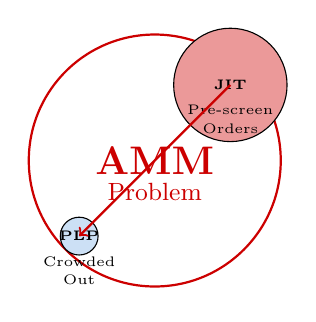
\begin{tikzpicture}[scale=0.8]
                % Problem visualization
                \draw[thick, parityred] (0,0) circle (2);
                \node[parityred] at (0,0) {\Large \textbf{AMM}};
                \node[parityred] at (0,-0.5) {\small Problem};
                
                % JIT LPs (large, dominant)
                \draw[fill=parityred!40] (1.2, 1.2) circle (0.9);
                \node[font=\tiny] at (1.2, 1.2) {\textbf{JIT}};
                \node[font=\tiny] at (1.2, 0.8) {Pre-screen};
                \node[font=\tiny] at (1.2, 0.5) {Orders};
                
                % PLPs (small, crowded out)
                \draw[fill=parityblue!20] (-1.2, -1.2) circle (0.3);
                \node[font=\tiny] at (-1.2, -1.2) {\textbf{PLP}};
                \node[font=\tiny] at (-1.2, -1.6) {Crowded};
                \node[font=\tiny] at (-1.2, -1.9) {Out};
                
                % Arrow showing crowding out
                \draw[->, thick, parityred] (1.2, 1.2) -- (-1.2, -1.2);
            \end{tikzpicture}
        \end{column}
    \end{columns}
\end{frame}

% Slide 5: Research Foundation - The Solution
\begin{frame}{Research Foundation: The Mathematical Solution}
    \begin{columns}
        \begin{column}{0.5\textwidth}
            \textbf{The Solution Framework:}
            \begin{itemize}
                \item \textcolor{paritygreen}{\textbf{Two-tiered fee structure}} with transfer rate λ\citecapponi
                \item \textcolor{paritygreen}{\textbf{Commitment-based classification}} (φ = 1 for PLP, φ = 0 for JIT)\citecapponi
                \item \textcolor{paritygreen}{\textbf{Fee redistribution}} from JIT to PLPs\citecapponi
            \end{itemize}
            
            \vspace{0.5cm}
            \textbf{Implementation Status:}
            \begin{itemize}
                \item \textcolor{paritygreen}{\checkmark} \textbf{Basic Detection}: JIT concentration monitoring\citeaquilina
                \item \textcolor{parityorange}{\textbf{In Progress}}: Elasticity calculation\citecapponi
                \item \textcolor{parityblue}{\textbf{Roadmap}}: Welfare optimization\citema
            \end{itemize}
        \end{column}
        \begin{column}{0.5\textwidth}
            \textbf{Mathematical Framework:}
            \begin{itemize}
                \item \textcolor{parityblue}{\textbf{Equilibrium Condition:}}
                \begin{itemize}
                    \item $\zeta_U > \zeta(f, \lambda, \pi)$\citecapponi
                    \item Ensures non-trivial SPNE exists
                \end{itemize}
                
                \item \textcolor{parityblue}{\textbf{Optimal Transfer Rate:}}
                \begin{itemize}
                    \item $\lambda^* = \max\{\lambda \in [0,1] : U(\pi,\lambda) \geq 0\}$\citecapponi
                    \item Maximizes passive LP utility
                \end{itemize}
                
                \item \textcolor{parityblue}{\textbf{Fee Distribution:}}
                \begin{itemize}
                    \item JIT: $\lambda \times$ (Pro-rata Share)\citecapponi
                    \item PLP: $(1-\lambda) \times$ (JIT Share) + Direct Share\citecapponi
                \end{itemize}
            \end{itemize}
        \end{column}
    \end{columns}
\end{frame}

\begin{frame}{The ParityTax-AMM Solution}
    \begin{columns}
        \begin{column}{0.6\textwidth}
            \textbf{Core Innovation:}
            \textcolor{parityblue}{\Large Sophisticated Fiscal Policy Framework}\citecapponi\citema
            
            \vspace{0.5cm}
            \textbf{Implementation Architecture:}
            \begin{itemize}
                \item \textcolor{paritygreen}{\textbf{IFiscalPolicy Interface}}
                \begin{itemize}
                    \item `remit()` - Fee redistribution mechanism\citecapponi
                    \item `calculateOptimalTax()` - Dynamic tax calculation\citecapponi
                    \item `accrueCredit()` - Commitment-based rewards\citecapponi
                \end{itemize}
                
                \item \textcolor{paritygreen}{\textbf{Event-Driven Processing}}
                \begin{itemize}
                    \item `onLiquidityOnSwap()` - Real-time liquidity events\citema
                    \item `onPriceImpact()` - Price impact monitoring\citema
                    \item Transient storage for gas optimization\citema
                \end{itemize}
                
                \item \textcolor{paritygreen}{\textbf{Developer Customization}}
                \begin{itemize}
                    \item Upgradable fiscal policy contracts\citema
                    \item Classical fiscal policy parallels\citeaquilina
                    \item Governance integration via `beforeInitialize`\citema
                \end{itemize}
            \end{itemize}
        \end{column}
        \begin{column}{0.4\textwidth}
            \textbf{Current Implementation Status:}
            \begin{itemize}
                \item \textcolor{paritygreen}{\checkmark} \textbf{Event Data Capture}
                \begin{itemize}
                    \item Real-time data storage\citema
                    \item Transient storage optimization\citema
                \end{itemize}
                
                \item \textcolor{parityblue}{\textbf{Roadmap}}
                \begin{itemize}
                    \item Credit accrual logic\citecapponi
                    \item Fee redistribution mechanism\citecapponi
                    \item Welfare optimization\citema
                \end{itemize}
            \end{itemize}
        \end{column}
    \end{columns}
\end{frame}


% Slide 3: Technical Architecture
\begin{frame}{Technical Architecture}
    \begin{columns}
        \begin{column}{0.45\textwidth}  % Reduced text column width
            \textbf{Core Components:}
            \begin{itemize}
                \item \textcolor{parityblue}{\textbf{ParityTaxHook}}
                \begin{itemize}
                    \item \footnotesize Main hook implementing fee distribution logic\citecapponi
                \end{itemize}
                
                \item \textcolor{parityblue}{\textbf{FiscalListeningPost}}
                \begin{itemize}
                    \item \footnotesize Reactive network bridge for real-time updates\citema
                \end{itemize}
                
                \item \textcolor{parityblue}{\textbf{Fiscal Policy Interface}}
                \begin{itemize}
                    \item \footnotesize Customizable taxation and reward logic\citecapponi
                \end{itemize}
                
                \item \textcolor{parityblue}{\textbf{Transient Storage}}
                \begin{itemize}
                    \item \footnotesize Gas-efficient parameter management\citema
                \end{itemize}
            \end{itemize}
            
            \vspace{0.3cm}
            \textbf{Key Features:}
            \begin{itemize}
                \item \footnotesize Event-driven architecture\citema
                \item \footnotesize Dual LP system (JIT vs PLP)\citecapponi
                \item \footnotesize Governance integration\citeaquilina
                \item \footnotesize Gas optimization\citema
            \end{itemize}
        \end{column}
        \begin{column}{0.55\textwidth}  % Increased image column width
            \begin{figure}
                \centering
                \includegraphics[width=\linewidth]{contextDiagram.excalidraw.png}  % Full column width
                \caption{ParityTax-AMM System Architecture}
                \label{fig:system_architecture}
            \end{figure}
        \end{column}
    \end{columns}
\end{frame}

% Slide 5: Developer Experience
\begin{frame}{Developer Experience: Classical Fiscal Policy Parallel}
    \begin{columns}
        \begin{column}{0.5\textwidth}
            \textbf{Government Fiscal Policy Analogy:}
            \begin{itemize}
                \item \textcolor{parityblue}{\textbf{Tax Collection}}: JIT LPs pay taxes on fee revenue\citeaquilina
                \item \textcolor{parityblue}{\textbf{Revenue Allocation}}: Tax revenue allocated to PLPs\citecapponi
                \item \textcolor{parityblue}{\textbf{Policy Customization}}: Different pool deployers implement different policies\citema
                \item \textcolor{parityblue}{\textbf{Governance}}: Policy parameters set through democratic processes\citeaquilina
            \end{itemize}
            
            \vspace{0.5cm}
            \textbf{Benefits:}
            \begin{itemize}
                \item Modular Design\citema
                \item Upgradeable (UUPS pattern)\citema
                \item Gas Optimized\citema
                \item Governance Ready\citeaquilina
            \end{itemize}
        \end{column}
        \begin{column}{0.5\textwidth}
            \textbf{Developer Customization:}
            \begin{lstlisting}[language=Solidity]
// Primary customization points
function accrueCredit(
    PoolId poolId, 
    bytes memory data
) external returns(uint256, uint256);

function calculateOptimalTax(
    PoolId poolId, 
    bytes memory data
) external returns(uint24);
            \end{lstlisting}
            
            \vspace{0.5cm}
            \textbf{Architecture Benefits:}
            \begin{itemize}
                \item Clean separation of concerns\citema
                \item Policy evolution without migration\citema
                \item Complex optimization without blocking transactions\citema
                \item Built-in governance mechanisms\citeaquilina
            \end{itemize}
        \end{column}
    \end{columns}
\end{frame}

% Slide 6: Implementation Status & Roadmap

% Slide 7: Impact & Benefits
\begin{frame}{Impact \& Benefits for the Ecosystem}
    \vspace{-0.1cm} % Adjust this value to move content up
    
    \begin{columns}
        \begin{column}{0.33\textwidth}
            \textbf{Liquidity Providers:}
            \begin{itemize}
                \item \textcolor{paritygreen}{\textbf{Equitable fee distribution}} between JIT and PLP\citecapponi
                \item \textcolor{paritygreen}{\textbf{Reduced competition}} through commitment mechanisms\citecapponi
                \item \textcolor{paritygreen}{\textbf{Predictable rewards}} based on contribution\citema
            \end{itemize}
        \end{column}
        \begin{column}{0.33\textwidth}
            \textbf{Pool Deployers:}
            \begin{itemize}
                \item \textcolor{parityblue}{\textbf{Customizable fiscal policies}} for different pool types\citema
                \item \textcolor{parityblue}{\textbf{Democratic control}} over policy parameters\citeaquilina
                \item \textcolor{parityblue}{\textbf{Real-time parameter adjustment}} for optimal outcomes\citema
            \end{itemize}
        \end{column}
        \begin{column}{0.33\textwidth}
            \textbf{Developers:}
            \begin{itemize}
                \item \textcolor{parityorange}{\textbf{Clean, modular architecture}}\citema
                \item \textcolor{parityorange}{\textbf{Comprehensive templates}} and documentation\citema
                \item \textcolor{parityorange}{\textbf{Gas-optimized implementation}}\citema
            \end{itemize}
        \end{column}
    \end{columns}
    
    \vspace{0.5cm} % Reduced spacing
    \begin{center}
        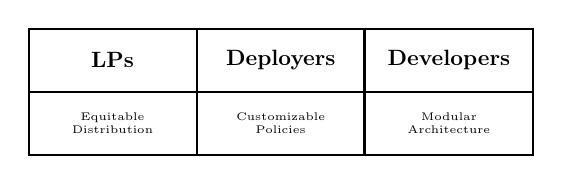
\begin{tikzpicture}[scale=0.8, transform shape] % Added scaling
            % Benefit matrix
            \draw[thick] (0,0) rectangle (8,2);
            \draw[thick] (2.67,0) -- (2.67,2);
            \draw[thick] (5.33,0) -- (5.33,2);
            \draw[thick] (0,1) -- (8,1);
            
            \node at (1.33, 1.5) {\textbf{LPs}};
            \node at (4, 1.5) {\textbf{Deployers}};
            \node at (6.67, 1.5) {\textbf{Developers}};
            
            \node[font=\tiny, align=center] at (1.33, 0.5) {Equitable\\Distribution};
            \node[font=\tiny, align=center] at (4, 0.5) {Customizable\\Policies};
            \node[font=\tiny, align=center] at (6.67, 0.5) {Modular\\Architecture};
        \end{tikzpicture}
    \end{center}
\end{frame}
% Slide 8: Call to Action
\begin{frame}{Next Steps \& Call to Action}
    \vspace{-0.2cm} % Adjust to fit content
    
    \begin{columns}
        \begin{column}{0.48\textwidth}
            \textbf{\textcolor{parityred}{High Priority TODOs:}}
            \begin{itemize}
                \item \textbf{Access Control}: Missing controls for critical functions
                \item \textbf{Interface Compliance}: Make \texttt{IFiscalPolicy} inherit \texttt{IERC4626}
                \item \textbf{Event Processing}: Complete \texttt{FiscalLogDispatcher}
                \item \textbf{Fiscal Policy}: Implement \texttt{\_accrueCredit()} logic
                \item \textbf{Data Structures}: Migrate to enumerable mappings
            \end{itemize}
        \end{column}
        \begin{column}{0.48\textwidth}
            \textbf{\textcolor{parityblue}{Medium Priority:}}
            \begin{itemize}
                \item Convert \texttt{LiquidityMetrics} to library
                \item Implement JIT resolver security checks
                \item Complete position commitment tests
            \end{itemize}
            
            \vspace{0.3cm}
            \textbf{\textcolor{paritygreen}{Call to Action:}}
            \begin{itemize}
                \item \textbf{Review code}: GitHub repository
                \item \textbf{Contribute}: Open to collaborators
                \item \textbf{Test}: Help with security auditing
                \item \textbf{Share}: Spread awareness in DeFi community
            \end{itemize}
        \end{column}
    \end{columns}
\end{frame}

% References slide
\begin{frame}{References}
    \tiny
    \begin{enumerate}
        \item \textbf{Aquilina, M., Foley, S., Gambacorta, L., \& Krekel, W.} (2024). 
              \textit{Decentralised dealers? Examining liquidity provision in decentralised exchanges}. 
              BIS Working Papers No. 1227.\\
              \textcolor{parityblue}{\url{https://www.bis.org/publ/work1227.pdf}}
        
        \vspace{0.2cm}
        \item \textbf{Capponi, A., Jia, R., \& Zhu, B.} (2024). 
              \textit{The Paradox Of Just-in-Time Liquidity in Decentralized Exchanges: More Providers Can Sometimes Mean Less Liquidity}. 
              arXiv:2311.18164.\\
              \textcolor{paritygreen}{\url{https://arxiv.org/abs/2311.18164}}
        
        \vspace{0.2cm}
        \item \textbf{Ma, J., \& Crapis, D.} (2024). 
              \textit{The Cost of Permissionless Liquidity Provision in Automated Market Makers}. 
              arXiv:2402.18256.\\
              \textcolor{parityorange}{\url{https://arxiv.org/abs/2402.18256}}
    \end{enumerate}
\end{frame}

% Thank you slide
\begin{frame}
    \begin{center}
        \Huge \textcolor{parityblue}{\textbf{Thank You!}}
        
        
        \vspace{1cm}
        \normalsize
        \textbf{ParityTax-AMM: Ensuring Equitable Fee Distribution in AMMs}
        
        \vspace{0.5cm}
        \textit{A Sophisticated Fiscal Policy Framework for AMM's}
    \end{center}
\end{frame}

\end{document}